%!TEX TS-program = PGF
%!TEX encoding = UTF-8
\documentclass{standalone}
\input{tikzstandalone}
\usepackage{hyperref}
\usepackage{pythontex}

\hypersetup{
        colorlinks = false,
	urlbordercolor = .1 .1 1,
	pdfborderstyle={/S/U/W 1} % liens soulignés, ne marche qu'avec acrobat
}


\newcommand\dessinecase[2][]{\draw[#1] (#2) ++(-.48, -.48) rectangle ++(.96, .96);}

\def\larg{1cm}
\def\haut{1cm}
\def\xoriginlanth{3.5}
\def\yoriginlanth{-1}

\sisetup{
round-mode = places, %pour contrôler le round-precision
%round-precision = 3
}


\begin{document}
%\begin{pycode}
%from chimie.periodikz import Tikz
%T = Tikz()
%
%T.add_symboles(with_style=['etat'])
%T.add_cases(with_style=['metal'])
%T.add_info(attr='chi', style='info1', format='$\\chi=\\num{{{}}}$')
%T.export('atomes2.tex')
%\end{pycode}

\fontfamily{cmr}
% helvetica : phv
% times : ptm
% latex : cmr
\fontsize{9}{10}\selectfont %default 10 12
%{size}{baselineskip} baseline-skip should be set to roughly 1.2x the font size


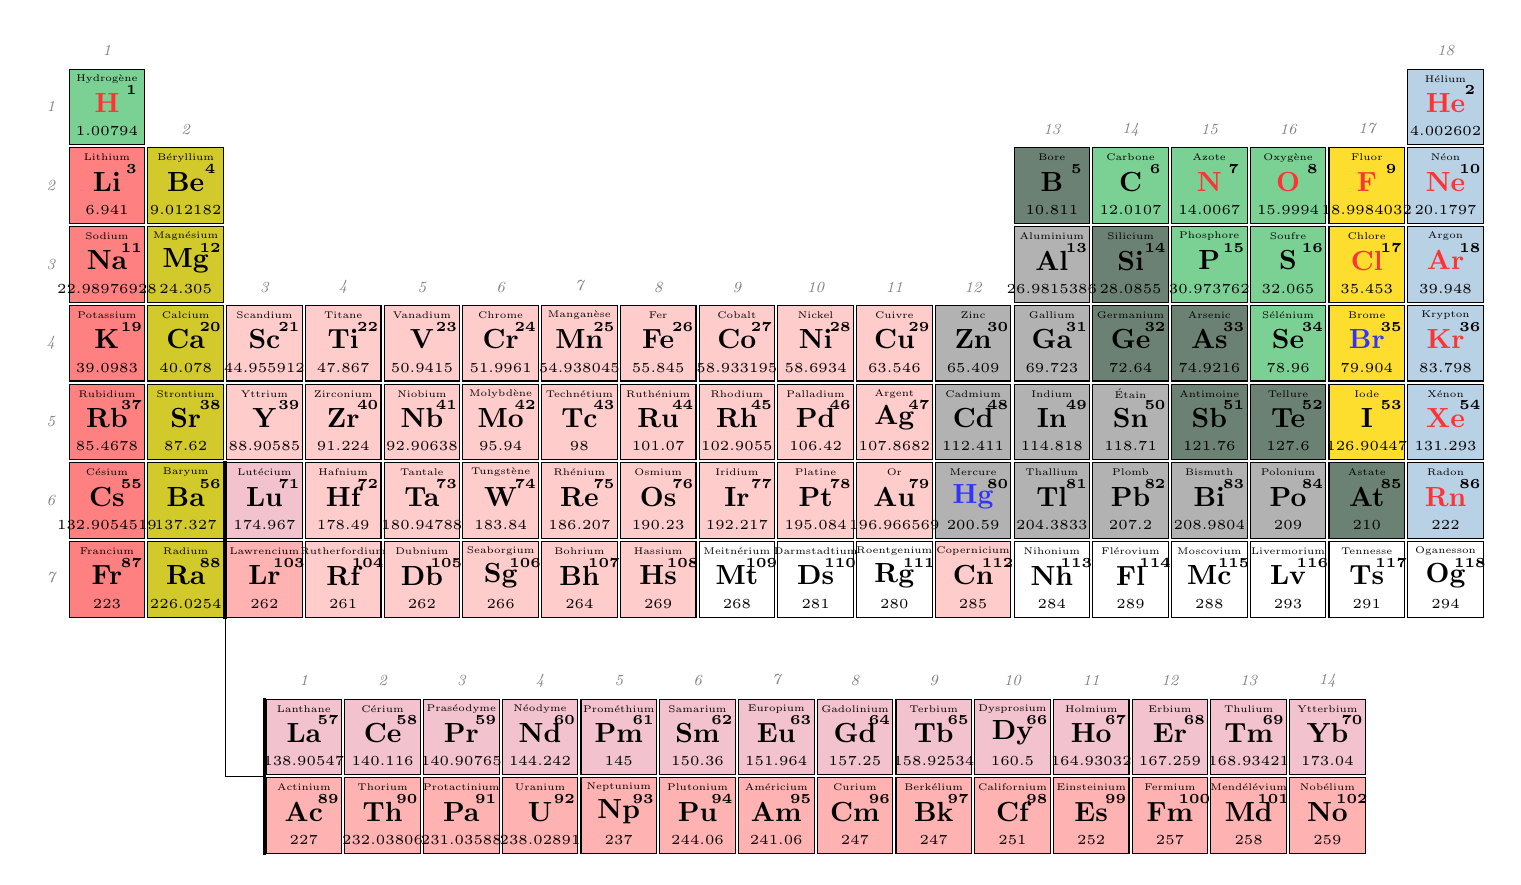
\begin{tikzpicture}[x=\larg, y=\haut,
	etat/.is choice,
	etat/g/.style={text=red!80!white},
	etat/l/.style={text=blue!80!white},
	etat/s/.style={black},
	groupe/.is choice,
	groupe/alcalin/.style={fill=red!50!white},
	groupe/alcalino-terreux/.style={fill=yellow!80!black},
	groupe/chalcogène/.style={},
	groupe/halogène/.style={fill=yellow!80!white!90!red},
	groupe/gaz noble/.style={fill=blue!20!white!90!green},
	groupe/lanthanide/.style={fill=red!20!white!95!blue},
	groupe/actinide/.style={fill=red!30!white},
	groupe/no/.style={},
	bloc/.is choice,
	bloc/s/.style={},
	bloc/p/.style={},
	bloc/d/.style={},
	bloc/f/.style={},
	origine/.is choice,
	origine/primordial/.style={},
	origine/désintégration/.style={},
	origine/synthétique/.style={},
	chi/.style={},
	radioactif/.style={},
	discovery/.style={},
	metal/.is choice,
	metal/no/.style={},
	metal/autre/.style={fill=green!80!yellow!70!blue!60!white},
	metal/alcalin/.style={fill=red!50!white},
	metal/alcalino-terreux/.style={fill=yellow!80!black},
	metal/métalloïde/.style={fill=red!25!green!70!blue!25!gray},
	metal/métal pauvre/.style={fill=gray!60!white},
	metal/métal de transition/.style={fill=red!20!white},
	metal/lanthanide/.style={fill=red!20!white!95!blue},
	metal/actinide/.style={fill=red!30!white},
	metal/unknown/.style={fill=white},
	titre colonne/.style={gray, scale=.7, node font={\itshape\footnotesize}, yshift=-.4\haut},
	titre ligne/.style={gray, scale=.7, node font={\itshape\footnotesize}, xshift=.4\larg},
	symbole/.style={node font={\bfseries\normalsize}, yshift=.05\haut},
	chi info/.style={right, node font={\tiny}, yshift=-.3\haut, xshift=-.5\larg},
	M info/.style={node font={\tiny}, yshift=-.3\haut, },
%	M info/.style={right, node font={\tiny}, yshift=-.3\haut, xshift=-.5\larg},
	nom/.style={scale=.7, node font={\tiny}, yshift=.5\haut, text centered},
	Z/.style={node font={\bfseries\tiny}, yshift=.2\haut, xshift=.3\larg}
]

\foreach \col in {1,...,18} {
	\foreach \ligne in {1,...,7} {
		\draw (\col, 7-\ligne) coordinate(\col-\ligne); %définit pour plus tard
	}
}

% titres
\foreach \col in {1,18} \draw (\col, 7) node[titre colonne]{\col};
\foreach \col in {2, 13, 14, 15, 16, 17} \draw (\col, 6) node[titre colonne]{\col};
\foreach \col in {3, ..., 12} \draw (\col, 4) node[titre colonne]{\col};
\foreach \ligne in {1,...,7} \draw (0, {(7-\ligne)}) node[titre ligne]{\ligne};

% lanthanides
\foreach \col in {1,...,14} {
	\draw (\xoriginlanth-1, \yoriginlanth) ++ (\col, 0) node[titre colonne]{\col};
	\draw ({\xoriginlanth+\col-1}, {\yoriginlanth-1}) coordinate(\col-L);
	\draw ({\xoriginlanth+\col-1}, {\yoriginlanth-2}) coordinate(\col-A);
}
\dessinecase[groupe=alcalin,
    metal=autre]{1-1}
\dessinecase[groupe=gaz noble,
    metal=no]{18-1}
\dessinecase[groupe=alcalin,
    metal=alcalin]{1-2}
\dessinecase[groupe=alcalino-terreux,
    metal=alcalino-terreux]{2-2}
\dessinecase[groupe=no,
    metal=métalloïde]{13-2}
\dessinecase[groupe=no,
    metal=autre]{14-2}
\dessinecase[groupe=no,
    metal=autre]{15-2}
\dessinecase[groupe=chalcogène,
    metal=autre]{16-2}
\dessinecase[groupe=halogène,
    metal=no]{17-2}
\dessinecase[groupe=gaz noble,
    metal=no]{18-2}
\dessinecase[groupe=alcalin,
    metal=alcalin]{1-3}
\dessinecase[groupe=alcalino-terreux,
    metal=alcalino-terreux]{2-3}
\dessinecase[groupe=no,
    metal=métal pauvre]{13-3}
\dessinecase[groupe=no,
    metal=métalloïde]{14-3}
\dessinecase[groupe=no,
    metal=autre]{15-3}
\dessinecase[groupe=chalcogène,
    metal=autre]{16-3}
\dessinecase[groupe=halogène,
    metal=no]{17-3}
\dessinecase[groupe=gaz noble,
    metal=no]{18-3}
\dessinecase[groupe=alcalin,
    metal=alcalin]{1-4}
\dessinecase[groupe=alcalino-terreux,
    metal=alcalino-terreux]{2-4}
\dessinecase[groupe=no,
    metal=métal de transition]{3-4}
\dessinecase[groupe=no,
    metal=métal de transition]{4-4}
\dessinecase[groupe=no,
    metal=métal de transition]{5-4}
\dessinecase[groupe=no,
    metal=métal de transition]{6-4}
\dessinecase[groupe=no,
    metal=métal de transition]{7-4}
\dessinecase[groupe=no,
    metal=métal de transition]{8-4}
\dessinecase[groupe=no,
    metal=métal de transition]{9-4}
\dessinecase[groupe=no,
    metal=métal de transition]{10-4}
\dessinecase[groupe=no,
    metal=métal de transition]{11-4}
\dessinecase[groupe=no,
    metal=métal pauvre]{12-4}
\dessinecase[groupe=no,
    metal=métal pauvre]{13-4}
\dessinecase[groupe=no,
    metal=métalloïde]{14-4}
\dessinecase[groupe=no,
    metal=métalloïde]{15-4}
\dessinecase[groupe=chalcogène,
    metal=autre]{16-4}
\dessinecase[groupe=halogène,
    metal=no]{17-4}
\dessinecase[groupe=gaz noble,
    metal=no]{18-4}
\dessinecase[groupe=alcalin,
    metal=alcalin]{1-5}
\dessinecase[groupe=alcalino-terreux,
    metal=alcalino-terreux]{2-5}
\dessinecase[groupe=no,
    metal=métal de transition]{3-5}
\dessinecase[groupe=no,
    metal=métal de transition]{4-5}
\dessinecase[groupe=no,
    metal=métal de transition]{5-5}
\dessinecase[groupe=no,
    metal=métal de transition]{6-5}
\dessinecase[groupe=no,
    metal=métal de transition]{7-5}
\dessinecase[groupe=no,
    metal=métal de transition]{8-5}
\dessinecase[groupe=no,
    metal=métal de transition]{9-5}
\dessinecase[groupe=no,
    metal=métal de transition]{10-5}
\dessinecase[groupe=no,
    metal=métal de transition]{11-5}
\dessinecase[groupe=no,
    metal=métal pauvre]{12-5}
\dessinecase[groupe=no,
    metal=métal pauvre]{13-5}
\dessinecase[groupe=no,
    metal=métal pauvre]{14-5}
\dessinecase[groupe=no,
    metal=métalloïde]{15-5}
\dessinecase[groupe=chalcogène,
    metal=métalloïde]{16-5}
\dessinecase[groupe=halogène,
    metal=no]{17-5}
\dessinecase[groupe=gaz noble,
    metal=no]{18-5}
\dessinecase[groupe=alcalin,
    metal=alcalin]{1-6}
\dessinecase[groupe=alcalino-terreux,
    metal=alcalino-terreux]{2-6}
\dessinecase[groupe=lanthanide,
    metal=lanthanide]{1-L}
\dessinecase[groupe=lanthanide,
    metal=lanthanide]{2-L}
\dessinecase[groupe=lanthanide,
    metal=lanthanide]{3-L}
\dessinecase[groupe=lanthanide,
    metal=lanthanide]{4-L}
\dessinecase[groupe=lanthanide,
    metal=lanthanide]{5-L}
\dessinecase[groupe=lanthanide,
    metal=lanthanide]{6-L}
\dessinecase[groupe=lanthanide,
    metal=lanthanide]{7-L}
\dessinecase[groupe=lanthanide,
    metal=lanthanide]{8-L}
\dessinecase[groupe=lanthanide,
    metal=lanthanide]{9-L}
\dessinecase[groupe=lanthanide,
    metal=lanthanide]{10-L}
\dessinecase[groupe=lanthanide,
    metal=lanthanide]{11-L}
\dessinecase[groupe=lanthanide,
    metal=lanthanide]{12-L}
\dessinecase[groupe=lanthanide,
    metal=lanthanide]{13-L}
\dessinecase[groupe=lanthanide,
    metal=lanthanide]{14-L}
\dessinecase[groupe=lanthanide,
    metal=lanthanide]{3-6}
\dessinecase[groupe=no,
    metal=métal de transition]{4-6}
\dessinecase[groupe=no,
    metal=métal de transition]{5-6}
\dessinecase[groupe=no,
    metal=métal de transition]{6-6}
\dessinecase[groupe=no,
    metal=métal de transition]{7-6}
\dessinecase[groupe=no,
    metal=métal de transition]{8-6}
\dessinecase[groupe=no,
    metal=métal de transition]{9-6}
\dessinecase[groupe=no,
    metal=métal de transition]{10-6}
\dessinecase[groupe=no,
    metal=métal de transition]{11-6}
\dessinecase[groupe=no,
    metal=métal pauvre]{12-6}
\dessinecase[groupe=no,
    metal=métal pauvre]{13-6}
\dessinecase[groupe=no,
    metal=métal pauvre]{14-6}
\dessinecase[groupe=no,
    metal=métal pauvre]{15-6}
\dessinecase[groupe=chalcogène,
    metal=métal pauvre]{16-6}
\dessinecase[groupe=halogène,
    metal=métalloïde]{17-6}
\dessinecase[groupe=gaz noble,
    metal=no]{18-6}
\dessinecase[groupe=alcalin,
    metal=alcalin]{1-7}
\dessinecase[groupe=alcalino-terreux,
    metal=alcalino-terreux]{2-7}
\dessinecase[groupe=actinide,
    metal=actinide]{1-A}
\dessinecase[groupe=actinide,
    metal=actinide]{2-A}
\dessinecase[groupe=actinide,
    metal=actinide]{3-A}
\dessinecase[groupe=actinide,
    metal=actinide]{4-A}
\dessinecase[groupe=actinide,
    metal=actinide]{5-A}
\dessinecase[groupe=actinide,
    metal=actinide]{6-A}
\dessinecase[groupe=actinide,
    metal=actinide]{7-A}
\dessinecase[groupe=actinide,
    metal=actinide]{8-A}
\dessinecase[groupe=actinide,
    metal=actinide]{9-A}
\dessinecase[groupe=actinide,
    metal=actinide]{10-A}
\dessinecase[groupe=actinide,
    metal=actinide]{11-A}
\dessinecase[groupe=actinide,
    metal=actinide]{12-A}
\dessinecase[groupe=actinide,
    metal=actinide]{13-A}
\dessinecase[groupe=actinide,
    metal=actinide]{14-A}
\dessinecase[groupe=actinide,
    metal=actinide]{3-7}
\dessinecase[groupe=no,
    metal=métal de transition]{4-7}
\dessinecase[groupe=no,
    metal=métal de transition]{5-7}
\dessinecase[groupe=no,
    metal=métal de transition]{6-7}
\dessinecase[groupe=no,
    metal=métal de transition]{7-7}
\dessinecase[groupe=no,
    metal=métal de transition]{8-7}
\dessinecase[groupe=no,
    metal=unknown]{9-7}
\dessinecase[groupe=no,
    metal=unknown]{10-7}
\dessinecase[groupe=no,
    metal=unknown]{11-7}
\dessinecase[groupe=no,
    metal=métal de transition]{12-7}
\dessinecase[groupe=no,
    metal=unknown]{13-7}
\dessinecase[groupe=no,
    metal=unknown]{14-7}
\dessinecase[groupe=no,
    metal=unknown]{15-7}
\dessinecase[groupe=chalcogène,
    metal=unknown]{16-7}
\dessinecase[groupe=halogène,
    metal=unknown]{17-7}
\dessinecase[groupe=gaz noble,
    metal=unknown]{18-7}
\draw (1-1) node[symbole, etat=g]{H};
\draw (18-1) node[symbole, etat=g]{He};
\draw (1-2) node[symbole, etat=s]{Li};
\draw (2-2) node[symbole, etat=s]{Be};
\draw (13-2) node[symbole, etat=s]{B};
\draw (14-2) node[symbole, etat=s]{C};
\draw (15-2) node[symbole, etat=g]{N};
\draw (16-2) node[symbole, etat=g]{O};
\draw (17-2) node[symbole, etat=g]{F};
\draw (18-2) node[symbole, etat=g]{Ne};
\draw (1-3) node[symbole, etat=s]{Na};
\draw (2-3) node[symbole, etat=s]{Mg};
\draw (13-3) node[symbole, etat=s]{Al};
\draw (14-3) node[symbole, etat=s]{Si};
\draw (15-3) node[symbole, etat=s]{P};
\draw (16-3) node[symbole, etat=s]{S};
\draw (17-3) node[symbole, etat=g]{Cl};
\draw (18-3) node[symbole, etat=g]{Ar};
\draw (1-4) node[symbole, etat=s]{K};
\draw (2-4) node[symbole, etat=s]{Ca};
\draw (3-4) node[symbole, etat=s]{Sc};
\draw (4-4) node[symbole, etat=s]{Ti};
\draw (5-4) node[symbole, etat=s]{V};
\draw (6-4) node[symbole, etat=s]{Cr};
\draw (7-4) node[symbole, etat=s]{Mn};
\draw (8-4) node[symbole, etat=s]{Fe};
\draw (9-4) node[symbole, etat=s]{Co};
\draw (10-4) node[symbole, etat=s]{Ni};
\draw (11-4) node[symbole, etat=s]{Cu};
\draw (12-4) node[symbole, etat=s]{Zn};
\draw (13-4) node[symbole, etat=s]{Ga};
\draw (14-4) node[symbole, etat=s]{Ge};
\draw (15-4) node[symbole, etat=s]{As};
\draw (16-4) node[symbole, etat=s]{Se};
\draw (17-4) node[symbole, etat=l]{Br};
\draw (18-4) node[symbole, etat=g]{Kr};
\draw (1-5) node[symbole, etat=s]{Rb};
\draw (2-5) node[symbole, etat=s]{Sr};
\draw (3-5) node[symbole, etat=s]{Y};
\draw (4-5) node[symbole, etat=s]{Zr};
\draw (5-5) node[symbole, etat=s]{Nb};
\draw (6-5) node[symbole, etat=s]{Mo};
\draw (7-5) node[symbole, etat=s]{Tc};
\draw (8-5) node[symbole, etat=s]{Ru};
\draw (9-5) node[symbole, etat=s]{Rh};
\draw (10-5) node[symbole, etat=s]{Pd};
\draw (11-5) node[symbole, etat=s]{Ag};
\draw (12-5) node[symbole, etat=s]{Cd};
\draw (13-5) node[symbole, etat=s]{In};
\draw (14-5) node[symbole, etat=s]{Sn};
\draw (15-5) node[symbole, etat=s]{Sb};
\draw (16-5) node[symbole, etat=s]{Te};
\draw (17-5) node[symbole, etat=s]{I};
\draw (18-5) node[symbole, etat=g]{Xe};
\draw (1-6) node[symbole, etat=s]{Cs};
\draw (2-6) node[symbole, etat=s]{Ba};
\draw (1-L) node[symbole, etat=s]{La};
\draw (2-L) node[symbole, etat=s]{Ce};
\draw (3-L) node[symbole, etat=s]{Pr};
\draw (4-L) node[symbole, etat=s]{Nd};
\draw (5-L) node[symbole, etat=s]{Pm};
\draw (6-L) node[symbole, etat=s]{Sm};
\draw (7-L) node[symbole, etat=s]{Eu};
\draw (8-L) node[symbole, etat=s]{Gd};
\draw (9-L) node[symbole, etat=s]{Tb};
\draw (10-L) node[symbole, etat=s]{Dy};
\draw (11-L) node[symbole, etat=s]{Ho};
\draw (12-L) node[symbole, etat=s]{Er};
\draw (13-L) node[symbole, etat=s]{Tm};
\draw (14-L) node[symbole, etat=s]{Yb};
\draw (3-6) node[symbole, etat=s]{Lu};
\draw (4-6) node[symbole, etat=s]{Hf};
\draw (5-6) node[symbole, etat=s]{Ta};
\draw (6-6) node[symbole, etat=s]{W};
\draw (7-6) node[symbole, etat=s]{Re};
\draw (8-6) node[symbole, etat=s]{Os};
\draw (9-6) node[symbole, etat=s]{Ir};
\draw (10-6) node[symbole, etat=s]{Pt};
\draw (11-6) node[symbole, etat=s]{Au};
\draw (12-6) node[symbole, etat=l]{Hg};
\draw (13-6) node[symbole, etat=s]{Tl};
\draw (14-6) node[symbole, etat=s]{Pb};
\draw (15-6) node[symbole, etat=s]{Bi};
\draw (16-6) node[symbole, etat=s]{Po};
\draw (17-6) node[symbole, etat=s]{At};
\draw (18-6) node[symbole, etat=g]{Rn};
\draw (1-7) node[symbole, etat=s]{Fr};
\draw (2-7) node[symbole, etat=s]{Ra};
\draw (1-A) node[symbole, etat=s]{Ac};
\draw (2-A) node[symbole, etat=s]{Th};
\draw (3-A) node[symbole, etat=s]{Pa};
\draw (4-A) node[symbole, etat=s]{U};
\draw (5-A) node[symbole, etat=s]{Np};
\draw (6-A) node[symbole, etat=s]{Pu};
\draw (7-A) node[symbole, etat=s]{Am};
\draw (8-A) node[symbole, etat=s]{Cm};
\draw (9-A) node[symbole, etat=s]{Bk};
\draw (10-A) node[symbole, etat=s]{Cf};
\draw (11-A) node[symbole, etat=s]{Es};
\draw (12-A) node[symbole, etat=s]{Fm};
\draw (13-A) node[symbole, etat=s]{Md};
\draw (14-A) node[symbole, etat=s]{No};
\draw (3-7) node[symbole, etat=s]{Lr};
\draw (4-7) node[symbole, etat=s]{Rf};
\draw (5-7) node[symbole, etat=s]{Db};
\draw (6-7) node[symbole, etat=s]{Sg};
\draw (7-7) node[symbole, etat=s]{Bh};
\draw (8-7) node[symbole, etat=s]{Hs};
\draw (9-7) node[symbole, etat=s]{Mt};
\draw (10-7) node[symbole, etat=s]{Ds};
\draw (11-7) node[symbole, etat=s]{Rg};
\draw (12-7) node[symbole, etat=s]{Cn};
\draw (13-7) node[symbole, etat=s]{Nh};
\draw (14-7) node[symbole, etat=s]{Fl};
\draw (15-7) node[symbole, etat=s]{Mc};
\draw (16-7) node[symbole, etat=s]{Lv};
\draw (17-7) node[symbole, etat=s]{Ts};
\draw (18-7) node[symbole, etat=s]{Og};
\draw (1-1) node[M info]{\num{1.00794}};
\draw (18-1) node[M info]{\num{4.002602}};
\draw (1-2) node[M info]{\num{6.941}};
\draw (2-2) node[M info]{\num{9.012182}};
\draw (13-2) node[M info]{\num{10.811}};
\draw (14-2) node[M info]{\num{12.0107}};
\draw (15-2) node[M info]{\num{14.0067}};
\draw (16-2) node[M info]{\num{15.9994}};
\draw (17-2) node[M info]{\num{18.9984032}};
\draw (18-2) node[M info]{\num{20.1797}};
\draw (1-3) node[M info]{\num{22.98976928}};
\draw (2-3) node[M info]{\num{24.305}};
\draw (13-3) node[M info]{\num{26.9815386}};
\draw (14-3) node[M info]{\num{28.0855}};
\draw (15-3) node[M info]{\num{30.973762}};
\draw (16-3) node[M info]{\num{32.065}};
\draw (17-3) node[M info]{\num{35.453}};
\draw (18-3) node[M info]{\num{39.948}};
\draw (1-4) node[M info]{\num{39.0983}};
\draw (2-4) node[M info]{\num{40.078}};
\draw (3-4) node[M info]{\num{44.955912}};
\draw (4-4) node[M info]{\num{47.867}};
\draw (5-4) node[M info]{\num{50.9415}};
\draw (6-4) node[M info]{\num{51.9961}};
\draw (7-4) node[M info]{\num{54.938045}};
\draw (8-4) node[M info]{\num{55.845}};
\draw (9-4) node[M info]{\num{58.933195}};
\draw (10-4) node[M info]{\num{58.6934}};
\draw (11-4) node[M info]{\num{63.546}};
\draw (12-4) node[M info]{\num{65.409}};
\draw (13-4) node[M info]{\num{69.723}};
\draw (14-4) node[M info]{\num{72.64}};
\draw (15-4) node[M info]{\num{74.9216}};
\draw (16-4) node[M info]{\num{78.96}};
\draw (17-4) node[M info]{\num{79.904}};
\draw (18-4) node[M info]{\num{83.798}};
\draw (1-5) node[M info]{\num{85.4678}};
\draw (2-5) node[M info]{\num{87.62}};
\draw (3-5) node[M info]{\num{88.90585}};
\draw (4-5) node[M info]{\num{91.224}};
\draw (5-5) node[M info]{\num{92.90638}};
\draw (6-5) node[M info]{\num{95.94}};
\draw (7-5) node[M info]{\num{98}};
\draw (8-5) node[M info]{\num{101.07}};
\draw (9-5) node[M info]{\num{102.9055}};
\draw (10-5) node[M info]{\num{106.42}};
\draw (11-5) node[M info]{\num{107.8682}};
\draw (12-5) node[M info]{\num{112.411}};
\draw (13-5) node[M info]{\num{114.818}};
\draw (14-5) node[M info]{\num{118.71}};
\draw (15-5) node[M info]{\num{121.76}};
\draw (16-5) node[M info]{\num{127.6}};
\draw (17-5) node[M info]{\num{126.90447}};
\draw (18-5) node[M info]{\num{131.293}};
\draw (1-6) node[M info]{\num{132.9054519}};
\draw (2-6) node[M info]{\num{137.327}};
\draw (1-L) node[M info]{\num{138.90547}};
\draw (2-L) node[M info]{\num{140.116}};
\draw (3-L) node[M info]{\num{140.90765}};
\draw (4-L) node[M info]{\num{144.242}};
\draw (5-L) node[M info]{\num{145}};
\draw (6-L) node[M info]{\num{150.36}};
\draw (7-L) node[M info]{\num{151.964}};
\draw (8-L) node[M info]{\num{157.25}};
\draw (9-L) node[M info]{\num{158.92534}};
\draw (10-L) node[M info]{\num{160.5}};
\draw (11-L) node[M info]{\num{164.93032}};
\draw (12-L) node[M info]{\num{167.259}};
\draw (13-L) node[M info]{\num{168.93421}};
\draw (14-L) node[M info]{\num{173.04}};
\draw (3-6) node[M info]{\num{174.967}};
\draw (4-6) node[M info]{\num{178.49}};
\draw (5-6) node[M info]{\num{180.94788}};
\draw (6-6) node[M info]{\num{183.84}};
\draw (7-6) node[M info]{\num{186.207}};
\draw (8-6) node[M info]{\num{190.23}};
\draw (9-6) node[M info]{\num{192.217}};
\draw (10-6) node[M info]{\num{195.084}};
\draw (11-6) node[M info]{\num{196.966569}};
\draw (12-6) node[M info]{\num{200.59}};
\draw (13-6) node[M info]{\num{204.3833}};
\draw (14-6) node[M info]{\num{207.2}};
\draw (15-6) node[M info]{\num{208.9804}};
\draw (16-6) node[M info]{\num{209}};
\draw (17-6) node[M info]{\num{210}};
\draw (18-6) node[M info]{\num{222}};
\draw (1-7) node[M info]{\num{223}};
\draw (2-7) node[M info]{\num{226.0254}};
\draw (1-A) node[M info]{\num{227}};
\draw (2-A) node[M info]{\num{232.03806}};
\draw (3-A) node[M info]{\num{231.03588}};
\draw (4-A) node[M info]{\num{238.02891}};
\draw (5-A) node[M info]{\num{237}};
\draw (6-A) node[M info]{\num{244.06}};
\draw (7-A) node[M info]{\num{241.06}};
\draw (8-A) node[M info]{\num{247}};
\draw (9-A) node[M info]{\num{247}};
\draw (10-A) node[M info]{\num{251}};
\draw (11-A) node[M info]{\num{252}};
\draw (12-A) node[M info]{\num{257}};
\draw (13-A) node[M info]{\num{258}};
\draw (14-A) node[M info]{\num{259}};
\draw (3-7) node[M info]{\num{262}};
\draw (4-7) node[M info]{\num{261}};
\draw (5-7) node[M info]{\num{262}};
\draw (6-7) node[M info]{\num{266}};
\draw (7-7) node[M info]{\num{264}};
\draw (8-7) node[M info]{\num{269}};
\draw (9-7) node[M info]{\num{268}};
\draw (10-7) node[M info]{\num{281}};
\draw (11-7) node[M info]{\num{280}};
\draw (12-7) node[M info]{\num{285}};
\draw (13-7) node[M info]{\num{284}};
\draw (14-7) node[M info]{\num{289}};
\draw (15-7) node[M info]{\num{288}};
\draw (16-7) node[M info]{\num{293}};
\draw (17-7) node[M info]{\num{291}};
\draw (18-7) node[M info]{\num{294}};
\draw (1-1) node[nom]{Hydrogène};
\draw (18-1) node[nom]{Hélium};
\draw (1-2) node[nom]{Lithium};
\draw (2-2) node[nom]{Béryllium};
\draw (13-2) node[nom]{Bore};
\draw (14-2) node[nom]{Carbone};
\draw (15-2) node[nom]{Azote};
\draw (16-2) node[nom]{Oxygène};
\draw (17-2) node[nom]{Fluor};
\draw (18-2) node[nom]{Néon};
\draw (1-3) node[nom]{Sodium};
\draw (2-3) node[nom]{Magnésium};
\draw (13-3) node[nom]{Aluminium};
\draw (14-3) node[nom]{Silicium};
\draw (15-3) node[nom]{Phosphore};
\draw (16-3) node[nom]{Soufre};
\draw (17-3) node[nom]{Chlore};
\draw (18-3) node[nom]{Argon};
\draw (1-4) node[nom]{Potassium};
\draw (2-4) node[nom]{Calcium};
\draw (3-4) node[nom]{Scandium};
\draw (4-4) node[nom]{Titane};
\draw (5-4) node[nom]{Vanadium};
\draw (6-4) node[nom]{Chrome};
\draw (7-4) node[nom]{Manganèse};
\draw (8-4) node[nom]{Fer};
\draw (9-4) node[nom]{Cobalt};
\draw (10-4) node[nom]{Nickel};
\draw (11-4) node[nom]{Cuivre};
\draw (12-4) node[nom]{Zinc};
\draw (13-4) node[nom]{Gallium};
\draw (14-4) node[nom]{Germanium};
\draw (15-4) node[nom]{Arsenic};
\draw (16-4) node[nom]{Sélénium};
\draw (17-4) node[nom]{Brome};
\draw (18-4) node[nom]{Krypton};
\draw (1-5) node[nom]{Rubidium};
\draw (2-5) node[nom]{Strontium};
\draw (3-5) node[nom]{Yttrium};
\draw (4-5) node[nom]{Zirconium};
\draw (5-5) node[nom]{Niobium};
\draw (6-5) node[nom]{Molybdène};
\draw (7-5) node[nom]{Technétium};
\draw (8-5) node[nom]{Ruthénium};
\draw (9-5) node[nom]{Rhodium};
\draw (10-5) node[nom]{Palladium};
\draw (11-5) node[nom]{Argent};
\draw (12-5) node[nom]{Cadmium};
\draw (13-5) node[nom]{Indium};
\draw (14-5) node[nom]{Étain};
\draw (15-5) node[nom]{Antimoine};
\draw (16-5) node[nom]{Tellure};
\draw (17-5) node[nom]{Iode};
\draw (18-5) node[nom]{Xénon};
\draw (1-6) node[nom]{Césium};
\draw (2-6) node[nom]{Baryum};
\draw (1-L) node[nom]{Lanthane};
\draw (2-L) node[nom]{Cérium};
\draw (3-L) node[nom]{Praséodyme};
\draw (4-L) node[nom]{Néodyme};
\draw (5-L) node[nom]{Prométhium};
\draw (6-L) node[nom]{Samarium};
\draw (7-L) node[nom]{Europium};
\draw (8-L) node[nom]{Gadolinium};
\draw (9-L) node[nom]{Terbium};
\draw (10-L) node[nom]{Dysprosium};
\draw (11-L) node[nom]{Holmium};
\draw (12-L) node[nom]{Erbium};
\draw (13-L) node[nom]{Thulium};
\draw (14-L) node[nom]{Ytterbium};
\draw (3-6) node[nom]{Lutécium};
\draw (4-6) node[nom]{Hafnium};
\draw (5-6) node[nom]{Tantale};
\draw (6-6) node[nom]{Tungstène};
\draw (7-6) node[nom]{Rhénium};
\draw (8-6) node[nom]{Osmium};
\draw (9-6) node[nom]{Iridium};
\draw (10-6) node[nom]{Platine};
\draw (11-6) node[nom]{Or};
\draw (12-6) node[nom]{Mercure};
\draw (13-6) node[nom]{Thallium};
\draw (14-6) node[nom]{Plomb};
\draw (15-6) node[nom]{Bismuth};
\draw (16-6) node[nom]{Polonium};
\draw (17-6) node[nom]{Astate};
\draw (18-6) node[nom]{Radon};
\draw (1-7) node[nom]{Francium};
\draw (2-7) node[nom]{Radium};
\draw (1-A) node[nom]{Actinium};
\draw (2-A) node[nom]{Thorium};
\draw (3-A) node[nom]{Protactinium};
\draw (4-A) node[nom]{Uranium};
\draw (5-A) node[nom]{Neptunium};
\draw (6-A) node[nom]{Plutonium};
\draw (7-A) node[nom]{Américium};
\draw (8-A) node[nom]{Curium};
\draw (9-A) node[nom]{Berkélium};
\draw (10-A) node[nom]{Californium};
\draw (11-A) node[nom]{Einsteinium};
\draw (12-A) node[nom]{Fermium};
\draw (13-A) node[nom]{Mendélévium};
\draw (14-A) node[nom]{Nobélium};
\draw (3-7) node[nom]{Lawrencium};
\draw (4-7) node[nom]{Rutherfordium};
\draw (5-7) node[nom]{Dubnium};
\draw (6-7) node[nom]{Seaborgium};
\draw (7-7) node[nom]{Bohrium};
\draw (8-7) node[nom]{Hassium};
\draw (9-7) node[nom]{Meitnérium};
\draw (10-7) node[nom]{Darmstadtium};
\draw (11-7) node[nom]{Roentgenium};
\draw (12-7) node[nom]{Copernicium};
\draw (13-7) node[nom]{Nihonium};
\draw (14-7) node[nom]{Flérovium};
\draw (15-7) node[nom]{Moscovium};
\draw (16-7) node[nom]{Livermorium};
\draw (17-7) node[nom]{Tennesse};
\draw (18-7) node[nom]{Oganesson};
\draw (1-1) node[Z]{1};
\draw (18-1) node[Z]{2};
\draw (1-2) node[Z]{3};
\draw (2-2) node[Z]{4};
\draw (13-2) node[Z]{5};
\draw (14-2) node[Z]{6};
\draw (15-2) node[Z]{7};
\draw (16-2) node[Z]{8};
\draw (17-2) node[Z]{9};
\draw (18-2) node[Z]{10};
\draw (1-3) node[Z]{11};
\draw (2-3) node[Z]{12};
\draw (13-3) node[Z]{13};
\draw (14-3) node[Z]{14};
\draw (15-3) node[Z]{15};
\draw (16-3) node[Z]{16};
\draw (17-3) node[Z]{17};
\draw (18-3) node[Z]{18};
\draw (1-4) node[Z]{19};
\draw (2-4) node[Z]{20};
\draw (3-4) node[Z]{21};
\draw (4-4) node[Z]{22};
\draw (5-4) node[Z]{23};
\draw (6-4) node[Z]{24};
\draw (7-4) node[Z]{25};
\draw (8-4) node[Z]{26};
\draw (9-4) node[Z]{27};
\draw (10-4) node[Z]{28};
\draw (11-4) node[Z]{29};
\draw (12-4) node[Z]{30};
\draw (13-4) node[Z]{31};
\draw (14-4) node[Z]{32};
\draw (15-4) node[Z]{33};
\draw (16-4) node[Z]{34};
\draw (17-4) node[Z]{35};
\draw (18-4) node[Z]{36};
\draw (1-5) node[Z]{37};
\draw (2-5) node[Z]{38};
\draw (3-5) node[Z]{39};
\draw (4-5) node[Z]{40};
\draw (5-5) node[Z]{41};
\draw (6-5) node[Z]{42};
\draw (7-5) node[Z]{43};
\draw (8-5) node[Z]{44};
\draw (9-5) node[Z]{45};
\draw (10-5) node[Z]{46};
\draw (11-5) node[Z]{47};
\draw (12-5) node[Z]{48};
\draw (13-5) node[Z]{49};
\draw (14-5) node[Z]{50};
\draw (15-5) node[Z]{51};
\draw (16-5) node[Z]{52};
\draw (17-5) node[Z]{53};
\draw (18-5) node[Z]{54};
\draw (1-6) node[Z]{55};
\draw (2-6) node[Z]{56};
\draw (1-L) node[Z]{57};
\draw (2-L) node[Z]{58};
\draw (3-L) node[Z]{59};
\draw (4-L) node[Z]{60};
\draw (5-L) node[Z]{61};
\draw (6-L) node[Z]{62};
\draw (7-L) node[Z]{63};
\draw (8-L) node[Z]{64};
\draw (9-L) node[Z]{65};
\draw (10-L) node[Z]{66};
\draw (11-L) node[Z]{67};
\draw (12-L) node[Z]{68};
\draw (13-L) node[Z]{69};
\draw (14-L) node[Z]{70};
\draw (3-6) node[Z]{71};
\draw (4-6) node[Z]{72};
\draw (5-6) node[Z]{73};
\draw (6-6) node[Z]{74};
\draw (7-6) node[Z]{75};
\draw (8-6) node[Z]{76};
\draw (9-6) node[Z]{77};
\draw (10-6) node[Z]{78};
\draw (11-6) node[Z]{79};
\draw (12-6) node[Z]{80};
\draw (13-6) node[Z]{81};
\draw (14-6) node[Z]{82};
\draw (15-6) node[Z]{83};
\draw (16-6) node[Z]{84};
\draw (17-6) node[Z]{85};
\draw (18-6) node[Z]{86};
\draw (1-7) node[Z]{87};
\draw (2-7) node[Z]{88};
\draw (1-A) node[Z]{89};
\draw (2-A) node[Z]{90};
\draw (3-A) node[Z]{91};
\draw (4-A) node[Z]{92};
\draw (5-A) node[Z]{93};
\draw (6-A) node[Z]{94};
\draw (7-A) node[Z]{95};
\draw (8-A) node[Z]{96};
\draw (9-A) node[Z]{97};
\draw (10-A) node[Z]{98};
\draw (11-A) node[Z]{99};
\draw (12-A) node[Z]{100};
\draw (13-A) node[Z]{101};
\draw (14-A) node[Z]{102};
\draw (3-7) node[Z]{103};
\draw (4-7) node[Z]{104};
\draw (5-7) node[Z]{105};
\draw (6-7) node[Z]{106};
\draw (7-7) node[Z]{107};
\draw (8-7) node[Z]{108};
\draw (9-7) node[Z]{109};
\draw (10-7) node[Z]{110};
\draw (11-7) node[Z]{111};
\draw (12-7) node[Z]{112};
\draw (13-7) node[Z]{113};
\draw (14-7) node[Z]{114};
\draw (15-7) node[Z]{115};
\draw (16-7) node[Z]{116};
\draw (17-7) node[Z]{117};
\draw (18-7) node[Z]{118};

\draw[very thick] (2.5, -.5) -- ++(0,2) (\xoriginlanth-.5, \yoriginlanth-.5) -- ++(0,-2);
\draw (2.5, -.5) |- (\xoriginlanth-.5, \yoriginlanth-1.5);
\end{tikzpicture}

\end{document}
